\chapter{Introdução}
\thispagestyle{empty}

A otimização combinatória é uma importante área relacionada à pesquisa operacional. Um problema de otimização combinatória consiste em encontrar uma solução ótima dentre um conjunto finito de soluções. Neste capítulo, o Problema do Caixeiro Viajante é apresentado, junto a uma breve discussão acerca de sua importância e dificuldade de resolução. Além disso, para que o problema possa ser expresso de forma simples e consistente, alguns conceitos básicos sobre grafos são abordados. 

\section{TSP}
O Problema do Caixeiro Viajante (\textit{Traveling Salesman Problem}, TSP) é um dos mais famosos problemas de otimização combinatória na literatura. Dado um conjunto de cidades, o TSP consiste em encontrar uma rota que visite todas elas de forma a minimizar a distância total percorrida\footnote{Minimizar a distância total percorrida é a ``função objetivo'' do problema.} (ou o tempo total de viagem). A Figura \ref{fig:instanciaTSP} apresenta um exemplo de instância do TSP, na qual há seis cidades dispostas em um espaço bidimensional. No exemplo, a distância entre as cidades 1 e 4 é de 118 km, enquanto a das cidades 1 e 3 é de 174 km. De posse das distâncias entre cada par de cidades, obtém-se algo semelhante à Tabela \ref{tab:tabelaDistancias}.

\begin{figure}
       \centering
        \scalebox{0.8}{
    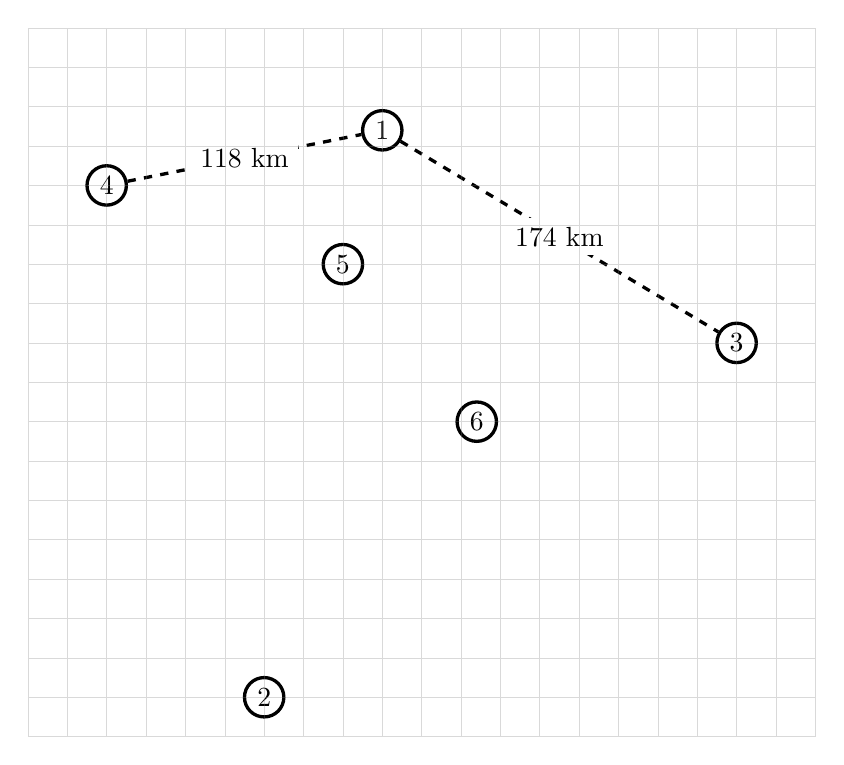
\begin{tikzpicture}
      
        \def\coordArray{-0.5/2.7,-2/-4.5,4/0,-4/2, -1/1, 0.7/-1};
        \foreach [count = \i] \x/\y in  \coordArray
        {
            \node[circle, draw=black, very thick,inner sep=0pt, minimum width=0.5cm] (\i) at (\x,\y) {\(\i\)};
        }
        
        \draw[dashed, very thick, opacity = 1.0] (1) -- node[fill=white]{\(174\) km} (3);
        \draw[dashed, very thick, opacity = 1.0] (4) -- node[fill=white]{\(118\) km} (1);
          \draw[help lines,step=0.5, opacity = 0.3](-5,-5)grid(5,4);
     %   \draw[->, >=latex, very thick] (1) -- (3) -- (5) -- (6) -- (2) -- (4) -- (1);
    \end{tikzpicture}
    }
    \caption{Exemplo de instância.}
    \label{fig:instanciaTSP}
\end{figure}

\begin{figure}[t]
    \centering
    \subfloat[Exemplo de solução viável.]{
    \scalebox{0.55}{
        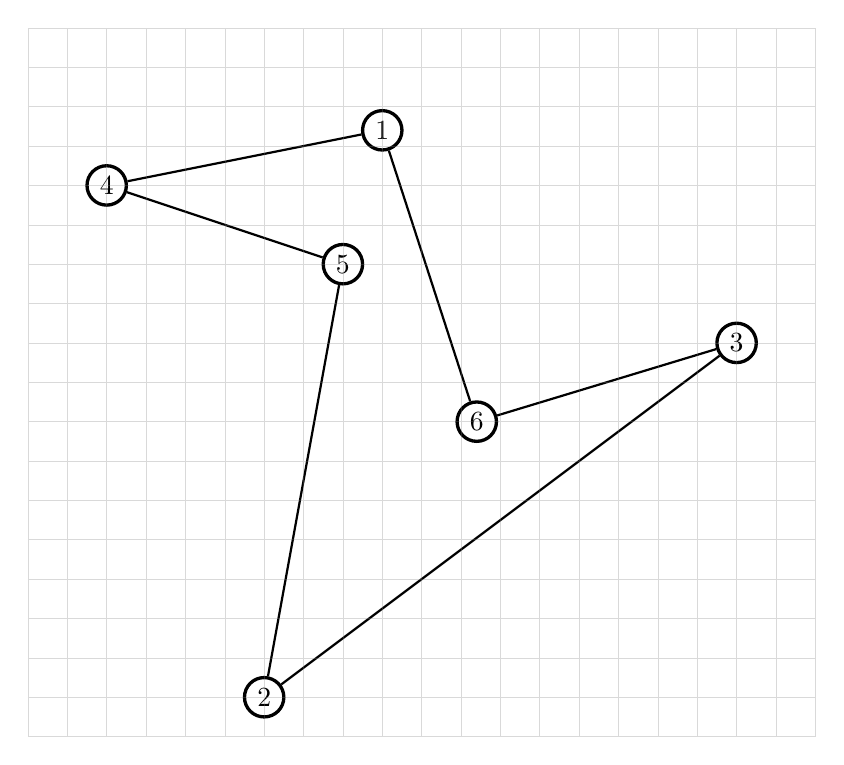
\begin{tikzpicture}
        \def\coordArray{-0.5/2.7,-2/-4.5,4/0,-4/2, -1/1, 0.7/-1};
        \foreach [count = \i] \x/\y in  \coordArray
        {
            \node[circle, draw=black, very thick,inner sep=0pt, minimum width=0.5cm] (\i) at (\x,\y) {\(\i\)};
        }
    
        
        \draw[-,>=latex, thick, opacity = 1.0] (1) -- (6);
        \draw[-,>=latex, thick, opacity = 1.0] (6) -- (3);
        \draw[-,>=latex, thick, opacity = 1.0] (3) --  (2);
        \draw[-,>=latex, thick, opacity = 1.0] (2) --  (5);
        \draw[-,>=latex, thick, opacity = 1.0] (5) --  (4);
        \draw[-,>=latex, thick, opacity = 1.0] (4) --  (1);
     %   \draw[->, >=latex, very thick] (1) -- (3) -- (5) -- (6) -- (2) -- (4) -- (1);
              \draw[help lines,step=0.5, opacity = 0.3](-5,-5)grid(5,4);

    \end{tikzpicture}
    }\label{fig:exemploSolucaoTSP1}}
    %\hspace{0.5cm}
    \subfloat[Exemplo de solução viável.]{
    \centering
    \scalebox{0.55}{
        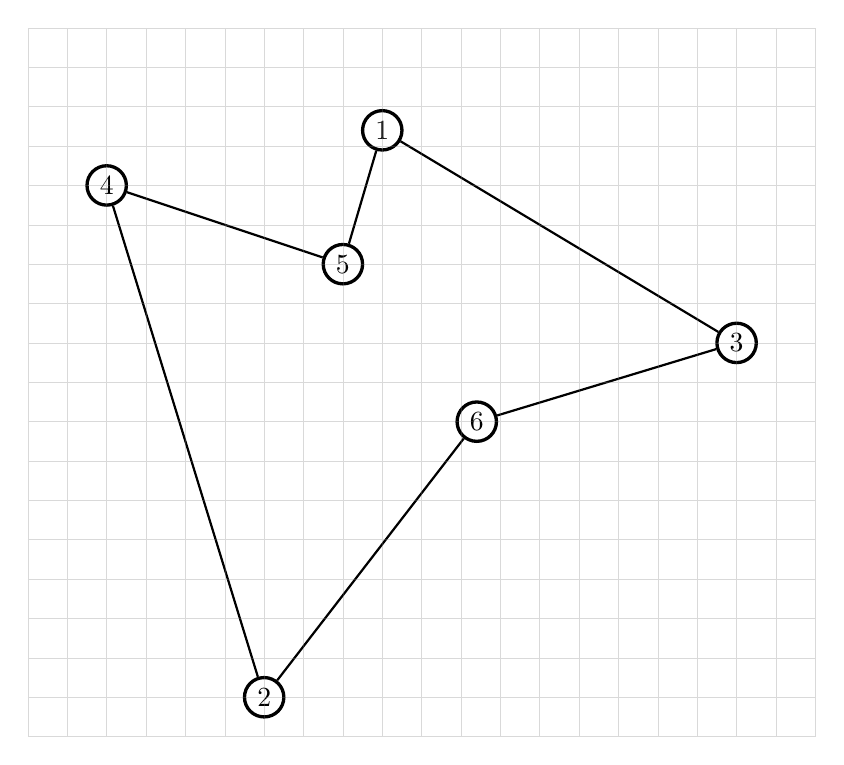
\begin{tikzpicture}
        \def\coordArray{-0.5/2.7,-2/-4.5,4/0,-4/2, -1/1, 0.7/-1};
        \foreach [count = \i] \x/\y in  \coordArray
        {
            \node[circle, draw=black, very thick,inner sep=0pt, minimum width=0.5cm] (\i) at (\x,\y) {\(\i\)};
        }
    
        
        \draw[-,>=latex, thick, opacity = 1.0] (1) -- (3);
        \draw[-,>=latex, thick, opacity = 1.0] (3) -- (6);
        \draw[-,>=latex, thick, opacity = 1.0] (6) --  (2);
        \draw[-,>=latex, thick, opacity = 1.0] (2) --  (4);
        \draw[-,>=latex, thick, opacity = 1.0] (4) --  (5);
        \draw[-,>=latex, thick, opacity = 1.0] (5) --  (1);
     %   \draw[->, >=latex, very thick] (1) -- (3) -- (5) -- (6) -- (2) -- (4) -- (1);
              \draw[help lines,step=0.5, opacity = 0.3](-5,-5)grid(5,4);

    \end{tikzpicture}
    }\label{fig:exemploSolucaoTSP2}}

    \caption{Exemplos de soluções viáveis.}
\end{figure}


\begin{table}[t]
\caption{Distâncias entre cada par de cidades (em km).}
\label{tab:tabelaDistancias}
\centering
\begin{tabular}{ccccccc}
\hline
\textbf{Cidade} & \(1\) & \(2\) & $3$ & $4$ & $5$ & $6$ \\ \hline
$1$             &       & 245   & 174 & 118 & 59  & 129 \\
$2$             &       &       & 250 & 226 & 186  & 147  \\
$3$             &       &       &     & 274 & 169 & 114  \\
$4$             &       &       &     &     & 105  & 185 \\
$5$             &       &       &     &     &     & 87  \\
$6$             &       &       &     &     &     &     \\ \hline
\end{tabular}
\end{table}


Uma solução válida (o termo ``viável'' será utilizado daqui em diante) para um TSP é uma sequência que visita cada cidade exatamente uma vez (um \textit{tour}). As figuras \ref{fig:exemploSolucaoTSP1} e \ref{fig:exemploSolucaoTSP2} mostram exemplos de soluções viáveis para a mesma instância. Ao verificar a Tabela \ref{tab:tabelaDistancias}, percebe-se que a distância total percorrida\footnote{Se a função objetivo do problema é minimizar a distância total percorrida, diz-se que a distância percorrida em uma solução é  o seu ``valor objetivo''.} na solução da Figura \ref{fig:exemploSolucaoTSP1} é de \(129 + 114 + 250 + 186 + 105 + 118 = 902\) km. A solução da Figura \ref{fig:exemploSolucaoTSP2}, por sua vez, possui uma distância total percorrida de \(174 + 114 + 147 + 226 + 105 + 59 = 825\) km, que é menor se comparada à solução da Figura \ref{fig:exemploSolucaoTSP1}, tornando-a preferível.



\subsection{Dificuldade}
Uma maneira de determinar a solução com o menor custo de viagem para uma instância é examinar todas as soluções possíveis. Note que diferentes soluções podem ser vistas como permutações do conjunto de cidades. Além disso, (i) não importa de onde se inicia o \textit{tour} (i.e., a sequência \((1, 3, 4, 5, 2, 1)\) é essencialmente igual à sequência \((2,1,3,4,5,2)\)); e (ii) percorrer um \textit{tour} no sentido anti-horário é igual a percorrê-lo no sentido horário\footnote{A versão do TSP abordada pressupõe que partir da cidade \(i\) para a cidade \(j\) é igual a partir da cidade \(j\) para a cidade \(i\). A variante na qual isso não é necessariamente verdade chama-se ATSP (\textit{Assymetrical Traveling Salesman Problem}).} (i.e., a sequência \((1,2,3,4,1)\) é igual à sequência \((1,4,3,2,1)\)). 

Então, se \(n\) é o número de cidades de uma determinada instância, o número de soluções distintas é \((n-1)!/2\). Dessa forma, resolver a instância descrita anteriormente exigiria examinar \((5!)/2 = 60\) soluções. Contudo, o TSP possui aplicações\footnote{O TSP é um subproblema de tarefas como a criação de trilhas que conectam pontos em placas de circuitos, sequenciamento de DNA, etc.} que envolvem instâncias com milhares (ou milhões) de cidades. Se \(n \geq 60\), o número de soluções possíveis ultrapassa o número estimado de átomos no universo. Portanto, examinar cada uma das soluções para instâncias desse tipo é impraticável computacionalmente.

\subsection{Abordagens}
Há duas maneiras de resolver problemas de otimização combinatória como o TSP: os métodos exatos e os métodos heurísticos. O primeiro visa obter soluções comprovadamente ótimas, enquanto o segundo busca obter soluções boas em um tempo razoável. Normalmente, os métodos exatos costumam ser mais lentos, e seu desempenho depende da existência de bons limitantes superiores\footnote{A solução da Figura \ref{fig:exemploSolucaoTSP2}, por exemplo, possui uma distância total de 825 km. Isso significa que uma solução ótima para essa instância não pode ter uma distância total maior que 825. Diz-se, portanto, que 825 é um ``limite superior''. Um método exato pode tirar proveito dessa informação. (\textit{upper bound}).}, que normalmente são providenciados pelos métodos heurísticos.

Embora o TSP seja um problema bem resolvido tanto de forma exata quanto heurística, ele serve como ponto de partida para o estudo de problemas mais avançados, como o Problema de Roteamento de Veículos e suas variantes, por compartilhar muitas de suas características com eles. O capítulo seguinte descreve uma abordagem heurística simples para resolver o TSP. A abordagem também é versátil, servindo como \textit{framework} para a resolução de vários outros problemas de otimização combinatória.

\section{Preliminares}
O algoritmo heurístico descrito no próximo capítulo deve ser implementado na linguagem C++. Para facilitar na compreensão do problema e no processo de implementação, alguns conceitos e observações são apresentados a seguir.  

\subsection{Grafos}
Sejam $V$ e $E$ conjuntos de vértices e arestas, respectivamente. O par \(G = (V, E)\) é considerado um grafo. Mais precisamente, \(E\) é um conjunto de pares \(\{i, j\}\) tais que \(i, j \in V, i \neq j\). Assim, qualquer conjunto de vértices ligados por arestas pode ser considerado um grafo. Um exemplo de grafo é mostrado na Figura \ref{fig:grafoNaoOrientado}. Nela, \(V = \{1,2,3,4,5\}\) e \(E = \{\{1,4\}, \{1,5\}, \{2,3\}, \{3,4\}, \{4,5\}, \{2,4\}, \{3,5\}\}\). Se todos os vértices estiverem conectados uns aos outros por arestas, \(G\) é um grafo completo. Um grafo completo com cinco vértices é ilustrado na Figura \ref{fig:grafoCompleto}.

\subsubsection{Grafo com pesos}
Se cada aresta $e = \{i,j\} \in E$ de um grafo estiver associada a um peso $c_{ij}$ (um número real qualquer), diz-se que esse grafo é um grafo com pesos. A Figura \ref{fig:grafoComPesos} ilustra um grafo com pesos em que $c_{2,3} = 3{,}14$, $c_{1,2} = 60$, $c_{3,5} = 42$, e $c_{4,5} = -1$.

\iffalse

\subsubsection{Grafo orientado}
Sejam \(V\) um conjunto de vértices e \(A\) um conjunto de arcos. \(G = (V,A)\) é um grafo orientado. Neste caso, \(A\) é um conjunto de pares ordenados (i.e., \((i,j) \neq (j,i)\)). Um exemplo de grafo orientado é mostrado na Figura \ref{fig:exemploGrafoOrientado}. 

\fi

% walk ?
\subsubsection{Passeio}
Dado um grafo $G = (V,E)$, a sequência alternada de vértices e arestas $v_0 e_0 v_1 e_1 \dots e_{k-1} v_k$ é considerada um passeio desde que toda aresta $e_i = \{v_i, v_{i+1}\}$ pertença a $E$. A Figura \ref{fig:grafoCaminho} contém um exemplo de um passeio percorrido sobre as arestas do grafo da Figura \ref{fig:grafoNaoOrientado}. Observe que tanto vértices quanto arestas podem ser percorridos mais de uma vez.

\subsubsection{Ciclo e ciclo Hamiltoniano}
Um ciclo é um passeio que começa e termina no mesmo vértice. Se todos os vértices no grafo são visitados exatamente uma vez, o ciclo é dito hamiltoniano. As figuras \ref{fig:grafoCiclo} e \ref{fig:grafoCicloHamiltoniano} ilustram um ciclo e um ciclo hamiltoniano, respectivamente.


\begin{figure}

\centering


\begin{subfigure}{.3\textwidth}
	\centering
	\scalebox{0.8}{
	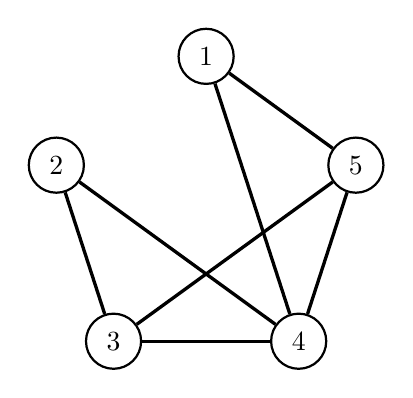
\begin{tikzpicture}
		%\draw[-{Latex[length=3mm,width=5mm]}] (0,0)--(2,0);	
		\node[circle, draw=black, inner sep=0pt, minimum size = 0.7cm, thick] (v1) at (0+90:2) {$1$};
		\node[circle, draw=black, inner sep=0pt, minimum size = 0.7cm, thick] (v2) at (72+90:2) {$2$};
		\node[circle, draw=black, inner sep=0pt, minimum size = 0.7cm, thick] (v3) at (144+90:2) {$3$};
		\node[circle, draw=black, inner sep=0pt, minimum size = 0.7cm, thick] (v4) at (216+90:2) {$4$};
		\node[circle, draw=black, inner sep=0pt, minimum size = 0.7cm, thick] (v5) at (288+90:2) {$5$};
		\draw[-, very thick] (v2) -- (v3);
		\draw[-, very thick] (v3) -- (v5);
		\draw[-, very thick] (v2) -- (v4);
		\draw[-, very thick] (v4) -- (v5);
		\draw[-, very thick] (v5) -- (v1);
		\draw[-, very thick] (v4) -- (v1);
		\draw[-, very thick] (v3) -- (v4);
	\end{tikzpicture}
}
	\caption{Grafo não orientado.}
	\label{fig:grafoNaoOrientado}
\end{subfigure}
\begin{subfigure}{.3\textwidth}
	\centering
	\scalebox{0.8}{
	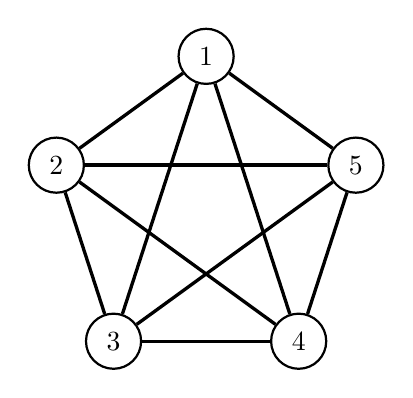
\begin{tikzpicture}
		%\draw[-{Latex[length=3mm,width=5mm]}] (0,0)--(2,0);	
		\node[circle, draw=black, inner sep=0pt, minimum size = 0.7cm, thick] (v1) at (0+90:2) {$1$};
		\node[circle, draw=black, inner sep=0pt, minimum size = 0.7cm, thick] (v2) at (72+90:2) {$2$};
		\node[circle, draw=black, inner sep=0pt, minimum size = 0.7cm, thick] (v3) at (144+90:2) {$3$};
		\node[circle, draw=black, inner sep=0pt, minimum size = 0.7cm, thick] (v4) at (216+90:2) {$4$};
		\node[circle, draw=black, inner sep=0pt, minimum size = 0.7cm, thick] (v5) at (288+90:2) {$5$};

		\foreach [count = \x] \n in {1,2,3,4,5}
		{
			\foreach [count = \y] \m in {1,2,3,4,5}
			{
				\ifnum \m > \n
				\draw[-, very thick] (v\n) -- (v\m);
				\fi
			}
		}
	\end{tikzpicture}
}
	\caption{Grafo completo.}
	\label{fig:grafoCompleto}
\end{subfigure}
\begin{subfigure}{.3\textwidth}
	\centering
	\scalebox{0.8}{
	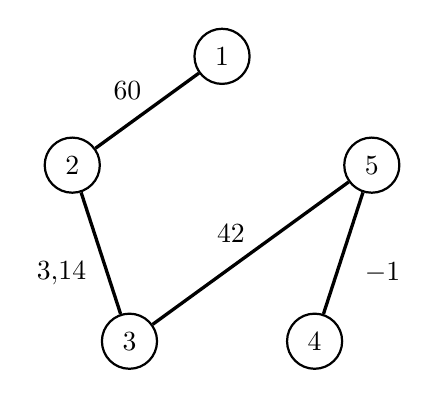
\begin{tikzpicture}
		%\draw[-{Latex[length=3mm,width=5mm]}] (0,0)--(2,0);	
		\node[circle, draw=black, inner sep=0pt, minimum size = 0.7cm, thick] (v1) at (0+90:2) {$1$};
		\node[circle, draw=black, inner sep=0pt, minimum size = 0.7cm, thick] (v2) at (72+90:2) {$2$};
		\node[circle, draw=black, inner sep=0pt, minimum size = 0.7cm, thick] (v3) at (144+90:2) {$3$};
		\node[circle, draw=black, inner sep=0pt, minimum size = 0.7cm, thick] (v4) at (216+90:2) {$4$};
		\node[circle, draw=black, inner sep=0pt, minimum size = 0.7cm, thick] (v5) at (288+90:2) {$5$};

		\draw[-, very thick] (v1) -- node[xshift=-0.25cm,yshift=0.25cm] {$60$} (v2) ;
		\draw[-, very thick] (v3) -- node[xshift=-0.25cm,yshift=0.25cm] {$42$} (v5) ;
		\draw[-, very thick] (v3) -- node[xshift=-0.5cm,yshift=-0.25cm] {$3{,}14$} (v2) ;
		\draw[-, very thick] (v4) -- node[xshift=0.5cm,yshift=-0.25cm] {$-1$} (v5) ;

	\end{tikzpicture}
}
	\caption{Grafo com pesos.}
	\label{fig:grafoComPesos}
\end{subfigure}
\begin{subfigure}{.3\textwidth}
	\centering
	\scalebox{0.8}{
	\begin{tikzpicture}
		%\draw[-{Latex[length=3mm,width=5mm]}] (0,0)--(2,0);	
		\node[circle, draw=black, inner sep=0pt, minimum size = 0.7cm, thick] (v1) at (0+90:2) {$1$};
		\node[circle, draw=black, inner sep=0pt, minimum size = 0.7cm, thick] (v2) at (72+90:2) {$2$};
		\node[circle, draw=black, inner sep=0pt, minimum size = 0.7cm, thick] (v3) at (144+90:2) {$3$};
		\node[circle, draw=black, inner sep=0pt, minimum size = 0.7cm, thick] (v4) at (216+90:2) {$4$};
		\node[circle, draw=black, inner sep=0pt, minimum size = 0.7cm, thick] (v5) at (288+90:2) {$5$};

		\draw[-, very thick, opacity = 0.25] (v3) -- (v5);
		\draw[-{Triangle}, line width = 0.05cm, color=blue] (v3) -- (v2);
		\draw[-{Triangle}, line width = 0.05cm, color=blue] (v2) -- (v4);
		\draw[-{Triangle}, line width = 0.05cm, color=blue] (v4) -- (v5);
		\draw[-, very thick, opacity = 0.25] (v5) -- (v1);
		\draw[-, very thick, opacity = 0.25] (v4) -- (v1);
		\draw[-, very thick, opacity = 0.25] (v3) -- (v4);
		\draw[-{Triangle[flex=0]}, line width = 0.05cm, color=blue] (v5) to [out=110, in=-10] (v1);
		\draw[-{Triangle[flex=0]}, line width = 0.05cm, color=blue] (v1) to [out=-70, in=170] (v5);
	\end{tikzpicture}
}
	\caption{Passeio.}
	\label{fig:grafoCaminho}
\end{subfigure}
\begin{subfigure}{.3\textwidth}
	\centering
	\scalebox{0.8}{
	\begin{tikzpicture}
		%\draw[-{Latex[length=3mm,width=5mm]}] (0,0)--(2,0);	
		\node[circle, draw=black, inner sep=0pt, minimum size = 0.7cm, thick] (v1) at (0+90:2) {$1$};
		\node[circle, draw=black, inner sep=0pt, minimum size = 0.7cm, thick] (v2) at (72+90:2) {$2$};
		\node[circle, draw=black, inner sep=0pt, minimum size = 0.7cm, thick] (v3) at (144+90:2) {$3$};
		\node[circle, draw=black, inner sep=0pt, minimum size = 0.7cm, thick] (v4) at (216+90:2) {$4$};
		\node[circle, draw=black, inner sep=0pt, minimum size = 0.7cm, thick] (v5) at (288+90:2) {$5$};

		\draw[-, very thick, opacity = 0.25] (v3) -- (v5);
		\draw[-{Triangle}, line width = 0.05cm, color=blue] (v3) -- (v2);
		\draw[-{Triangle}, line width = 0.05cm, color=blue] (v2) -- (v4);
		\draw[-, very thick, opacity = 0.25] (v4) -- (v5);
		\draw[-, very thick, opacity = 0.25] (v5) -- (v1);
		\draw[-, very thick, opacity = 0.25] (v4) -- (v1);
		\draw[-{Triangle}, line width = 0.05cm, color=blue] (v4) -- (v3);
	\end{tikzpicture}
}
	\caption{Ciclo.}
	\label{fig:grafoCiclo}
\end{subfigure}
\begin{subfigure}{.3\textwidth}
	\centering
	\scalebox{0.8}{
	\begin{tikzpicture}
		%\draw[-{Latex[length=3mm,width=5mm]}] (0,0)--(2,0);	
		\node[circle, draw=black, inner sep=0pt, minimum size = 0.7cm, thick] (v1) at (0+90:2) {$1$};
		\node[circle, draw=black, inner sep=0pt, minimum size = 0.7cm, thick] (v2) at (72+90:2) {$2$};
		\node[circle, draw=black, inner sep=0pt, minimum size = 0.7cm, thick] (v3) at (144+90:2) {$3$};
		\node[circle, draw=black, inner sep=0pt, minimum size = 0.7cm, thick] (v4) at (216+90:2) {$4$};
		\node[circle, draw=black, inner sep=0pt, minimum size = 0.7cm, thick] (v5) at (288+90:2) {$5$};

		\draw[-{Triangle}, line width = 0.05cm, color=blue] (v5) -- (v3);
		\draw[-{Triangle}, line width = 0.05cm, color=blue] (v3) -- (v2);
		\draw[-{Triangle}, line width = 0.05cm, color=blue] (v2) -- (v4);
		\draw[-, very thick, opacity = 0.25] (v4) -- (v5);
		\draw[-{Triangle}, line width = 0.05cm, color=blue] (v1) -- (v5);
		\draw[-{Triangle}, line width = 0.05cm, color=blue] (v4) -- (v1);
		\draw[-, very thick, opacity = 0.25] (v4) -- (v3);
	\end{tikzpicture}
}
	\caption{Ciclo hamiltoniano.}
	\label{fig:grafoCicloHamiltoniano}
\end{subfigure}
	\caption{Exemplos de grafos, caminhos e ciclos.}
	\label{fig:grafoExemplos}
\end{figure}



\subsection{Representação do TSP através de grafos}
Uma instância do TSP pode ser vista como um grafo completo com pesos, no qual cada nó corresponde a uma cidade, e cada aresta está associada a um custo que representa a distância entre as duas cidades correspondentes. Resolver o TSP equivale a encontrar o ciclo hamiltoniano nesse grafo cujo custo total (a soma dos pesos das arestas no ciclo) é o menor possível. 

O grafo citado pode, ainda, ser representado por uma matriz $M$, na qual o elemento $M_{ij} = c_{ij}$ equivale ao peso da aresta $\{i,j\}$. Por conter informações sobre as arestas, que consistem em pares de vértices adjacentes, diz-se que $M$ é uma matriz de adjacência.

\subsection{Leitor de instâncias}
Alguns arquivos de instâncias e o código de um leitor de instâncias se encontram neste link: \url{https://github.com/cvneves/kit-opt/tree/master/GILS-RVND-TSP/leitor-instancias}. O leitor computa a matriz de adjacência da instância, representando-a através do \textit{array} bidimensional \texttt{matrizAdj}. Note que os custos são indexados a partir de 1. Logo, se uma instância contém 14 cidades, a distância entre a primeira e a última cidade é \texttt{matrizAdj[1][14]} (ou \texttt{matrizAdj[14][1]}). 

\subsection{\textit{Standard Template Library}}
O uso do paradigma de programação orientada a objetos não é obrigatório. Contudo, para facilitar a implementação das estruturas de dados e rotinas necessárias no algoritmo, recomenda-se o estudo dos componentes \texttt{vector} e \texttt{sort()} da \textit{Standard Template Library} (STL). O trecho de código abaixo mostra como as soluções do TSP podem ser representadas. 

\begin{lstlisting}[style=cplusplusListStyle] 
typedef struct Solucao{
    vector<int> sequencia;
    double valorObj;
} Solucao;

// Exemplo de inicializacao 
Solucao s1 = {{1,6,3,2,5,4,1}, 0};

// Iterando pelos vertices da solucao 
void exibirSolucao(Solucao *s)
{
    for(int i = 0; i < s->sequencia.size() - 1; i++)
        std::cout << s->sequencia[i] << " -> ";
    std::cout << s->sequencia.back() << std::endl;
}

exibirSolucao(&s1);
// RESULTADO: "1 -> 6 -> 3 -> 2 -> 5 -> 4 -> 1" 

// Inicializando uma solucao vazia 
Solucao s2 = {{}, 0.0};
// Adicionando vertices na solucao 
s2.push_back(1);
s2.push_back(3);
s2.push_back(1);
exibirSolucao(&s2);
// RESULTADO: "1 -> 3 -> 1"
s2.insert(s2.begin() + 1, 4);
s2.insert(s2.end() - 1, 5);
s2.insert(s2.begin() + 2, 2);
exibirSolucao(&s2);
// RESULTADO: "1 -> 4 -> 2 -> 3 -> 5 -> 1"

void calcularValorObj(Solucao *s){
    s->valorObj = 0;
    for(int i = 0; i < s->sequencia.size() - 1; i++)
        s->valorObj += matrizAdj[s->sequencia[i]][s->sequencia[i+1]];
}
\end{lstlisting}


\subsection{Valores ótimos}
O valor ótimo de custo das instâncias fornecidas já foi determinado por meio de métodos exatos. Uma lista com esses valores --- que devem ser consultados para determinar a eficácia da implementação do algoritmo --- se encontra neste link: \url{http://comopt.ifi.uni-heidelberg.de/software/TSPLIB95/STSP.html}.

Depois de implementado, o algoritmo deve ser capaz de obter o valor ótimo para instâncias de até 300 cidades na maioria das vezes em que é executado\footnote{Além de não garantir a obtenção de uma solução ótima, o algoritmo não é determinístico. Por isso, determinar a robustez e velocidade de sua implementação exige testá-lo extensivamente.}.
